% * Week 2. (Aug 3) Business Analytics and Statistical Learning. Ch2. (Rob & Souhaib)
%   - Lecture 3: More on R and statistical learning. 
%   - Lab 2: 
%   - Lecture 4: Assessing model accuracy. Bias-variance tradeoff

%   Content: 
%     - Statistics? Machine learning? data mining? data science? Analytics? 
%     - The four V’s of big data/data science
%     - Analytics and data science jobs: “By 2018, the US could face a shortage of up to 190.000 workers with analytical skills” McKinsey


\documentclass[14pt]{beamer}
\usepackage{pgf,tikz,pgfpages,amsmath,bm,fancyvrb,animate}
\usepackage{graphicx,bera,booktabs}
\usepackage[australian]{babel}
\usepackage[utf8]{inputenc}

\usetheme{Monash}
\def\biz{\begin{itemize}[<+-| alert@+>]}
\def\eiz{\end{itemize}}
\def\ben{\begin{enumerate}[<+-| alert@+>]}
\def\een{\end{enumerate}}

\graphicspath{{../figures/}{../figures/book_figures/Chapter5/}}


\title[2. The Bootstrap]{Business Analytics}
\author{2. The Bootstrap}


\DefineShortVerb{\"}
\def\FancyVerbFormatCom{\color[rgb]{0.6,0,1}\relax}


\begin{document}

\begin{frame}[plain]{}
\maketitle
\begin{textblock}{11}(0.5,1.19){\color{white}\large
\textbf{ETC3250}}
\end{textblock}
\end{frame}

\begin{frame}[plain]{What is the bootstrap?}
%
The bootstrap is a flexible statistical tool to \textbf{quantify the uncertainty} associated with a \emph{given estimator} or \emph{statistical learning method}.
\begin{center}
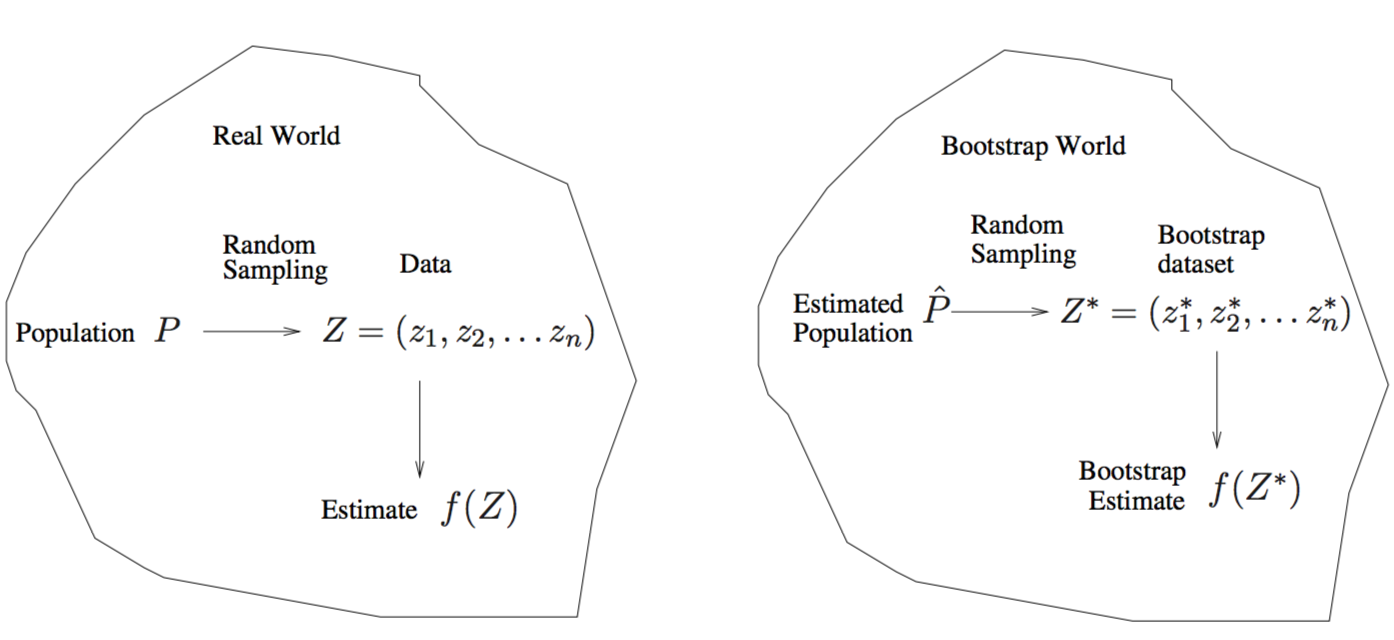
\includegraphics[width=1\textwidth]{general-bootstrap}	
\end{center}
\end{frame}


\begin{frame}[plain]{The bootstrap procedure}


mention sampling distribution

parametric vs nonparametric bootstrap

\end{frame}

\begin{frame}[plain]{Accuracy of the sample median}

Show the difference between standard error for the mean with formula and with bootstrap

Mention that this is not available in other cases

\begin{itemize}
	\item 
\end{itemize}
\end{frame}

\begin{frame}[plain]{Another example}

\begin{itemize}
	\item
\end{itemize}
\end{frame}

\begin{frame}[plain]{What is the bootstrap?}

\begin{itemize}
	\item  The bootstrap allows us to use a computer to mimic the process of obtaining new data sets, so that we can estimate the variability of our estimate without generating additional samples
	\item Rather than repeatedly obtaining independent data sets
from the population, we instead obtain distinct data sets (with the same size as our original dataset) by repeatedly sampling observations from the original data set with replacement.
	\item Other bootstrap procedures: parametric bootstrap, bootstrap for time series, bagging, etc.
\end{itemize}
\end{frame}

\begin{frame}[plain]{Illustration of the bootstrap}

\begin{center}
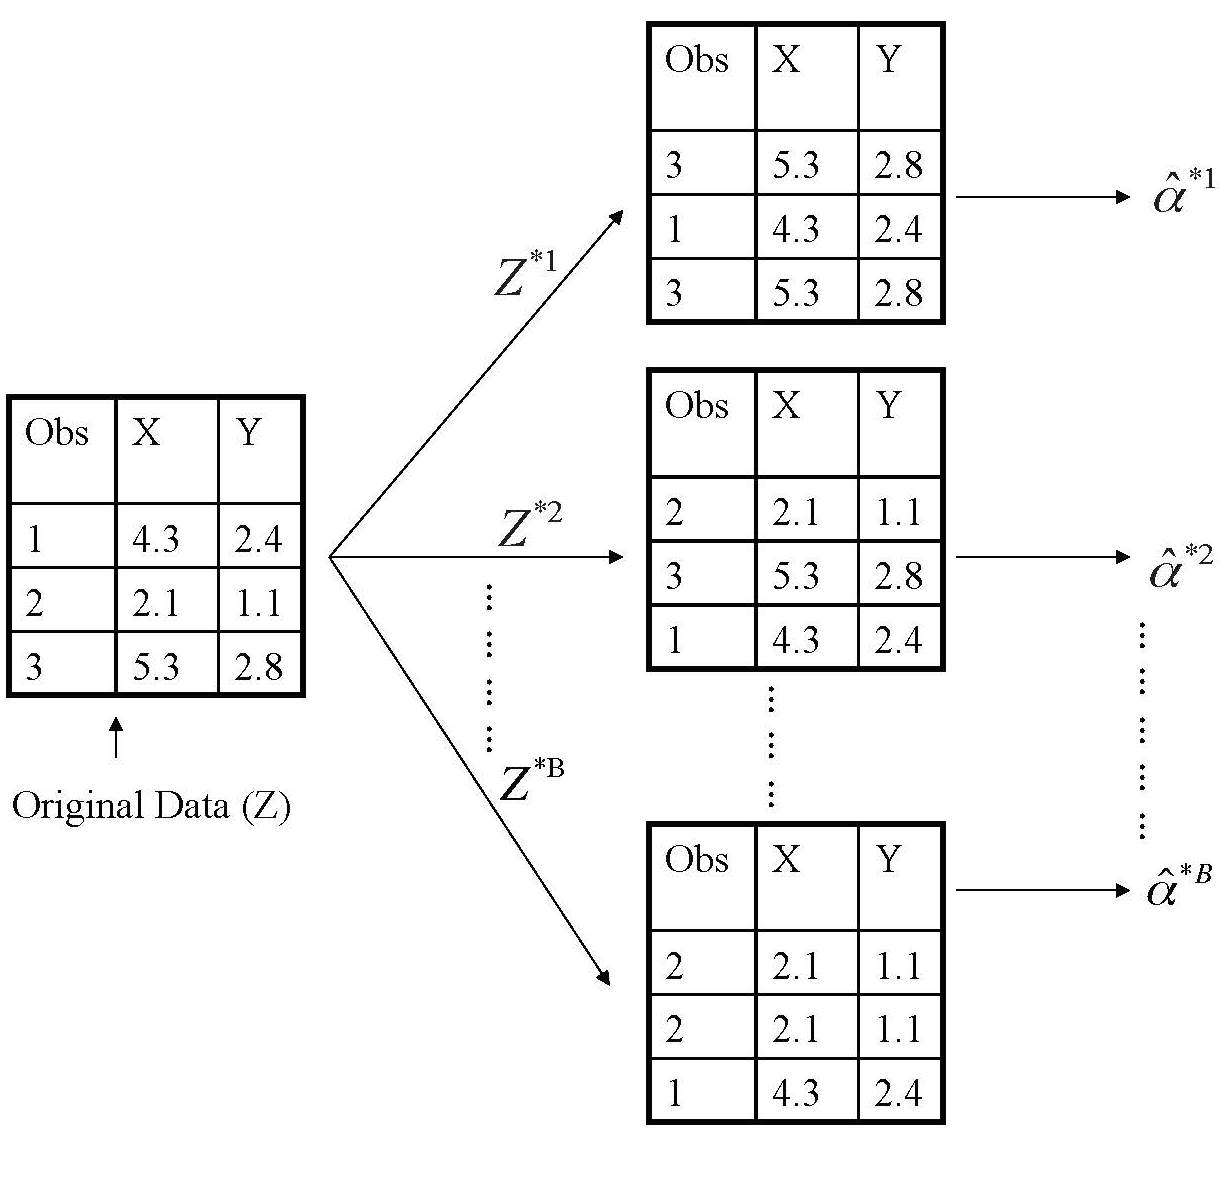
\includegraphics[width=.7\textwidth]{5-11.png}	
\end{center}
\end{frame}

\begin{frame}[plain]{Prediction error estimation?}

Write cross-validation formula and bootstrap formula (7.54 in ESL)
that crossvalidation
explicitly uses non-overlapping data for the training and test
samples.

\end{frame}

\begin{frame}[plain]{Prediction error estimation?}
%
Each of these bootstrap data sets is created by sampling with replacement, and is the same size as our original dataset. As a result some observations may appear more than once in a given bootstrap data set and some not at all.

\begin{align*}
	&\text{P}(\text{observation~} i \in \text{~bootstrap sample~} b) \\
	&= 1 - (1 - \frac1n)^n \\
	&\approx 1 - \frac1e \\
	&= 0.632
\end{align*}

\end{frame}






\end{document}